\section{Methods}
The Ferienakademie has many methods in its arsenal to garner the curiosity of students. In this section we want to present some of them. Furthermore, we want to take a look at how they are applied.
\subsection{Courses}
Without doubt, the main method are the courses themselves. The Ferienakademie lets the students choose from a wide variety of courses from a plethora of disciplines -- informatics, mathematics, medical engineering, psychology, philosophy, etc. The group size usually varies between 10-20 students. 

The typical structure of the course is the following: Depending on the core focus of a course, participants prepare a talk for a specific topic before the start of the academy. Quite a few courses consist of a group project. While students still might prepare a talk, they work on specific tasks in groups during their time in Sarntal. In 2015, for example, course 2 developed apps for iOS to enhance the quality of life, while course 5 created a game based on multiphysics simulation using the Xbox Kinect. 

In both cases, the small size of the group, the close interaction with the corresponding professors and the motivation of each participating student (and also the non-existent pressure of grading) creates a special atmosphere which leads to exciting discussions that extend beyond the workspace. (Rumours exist that whole game ideas were developed, discarded and reinvented during hikes.) % :D tap me a beer bro

Examples of both types of courses are shown in \autoref{fig:presentation} and \autoref{fig:project}.
\begin{figure}[ht]%
 	\begin{center}%
 		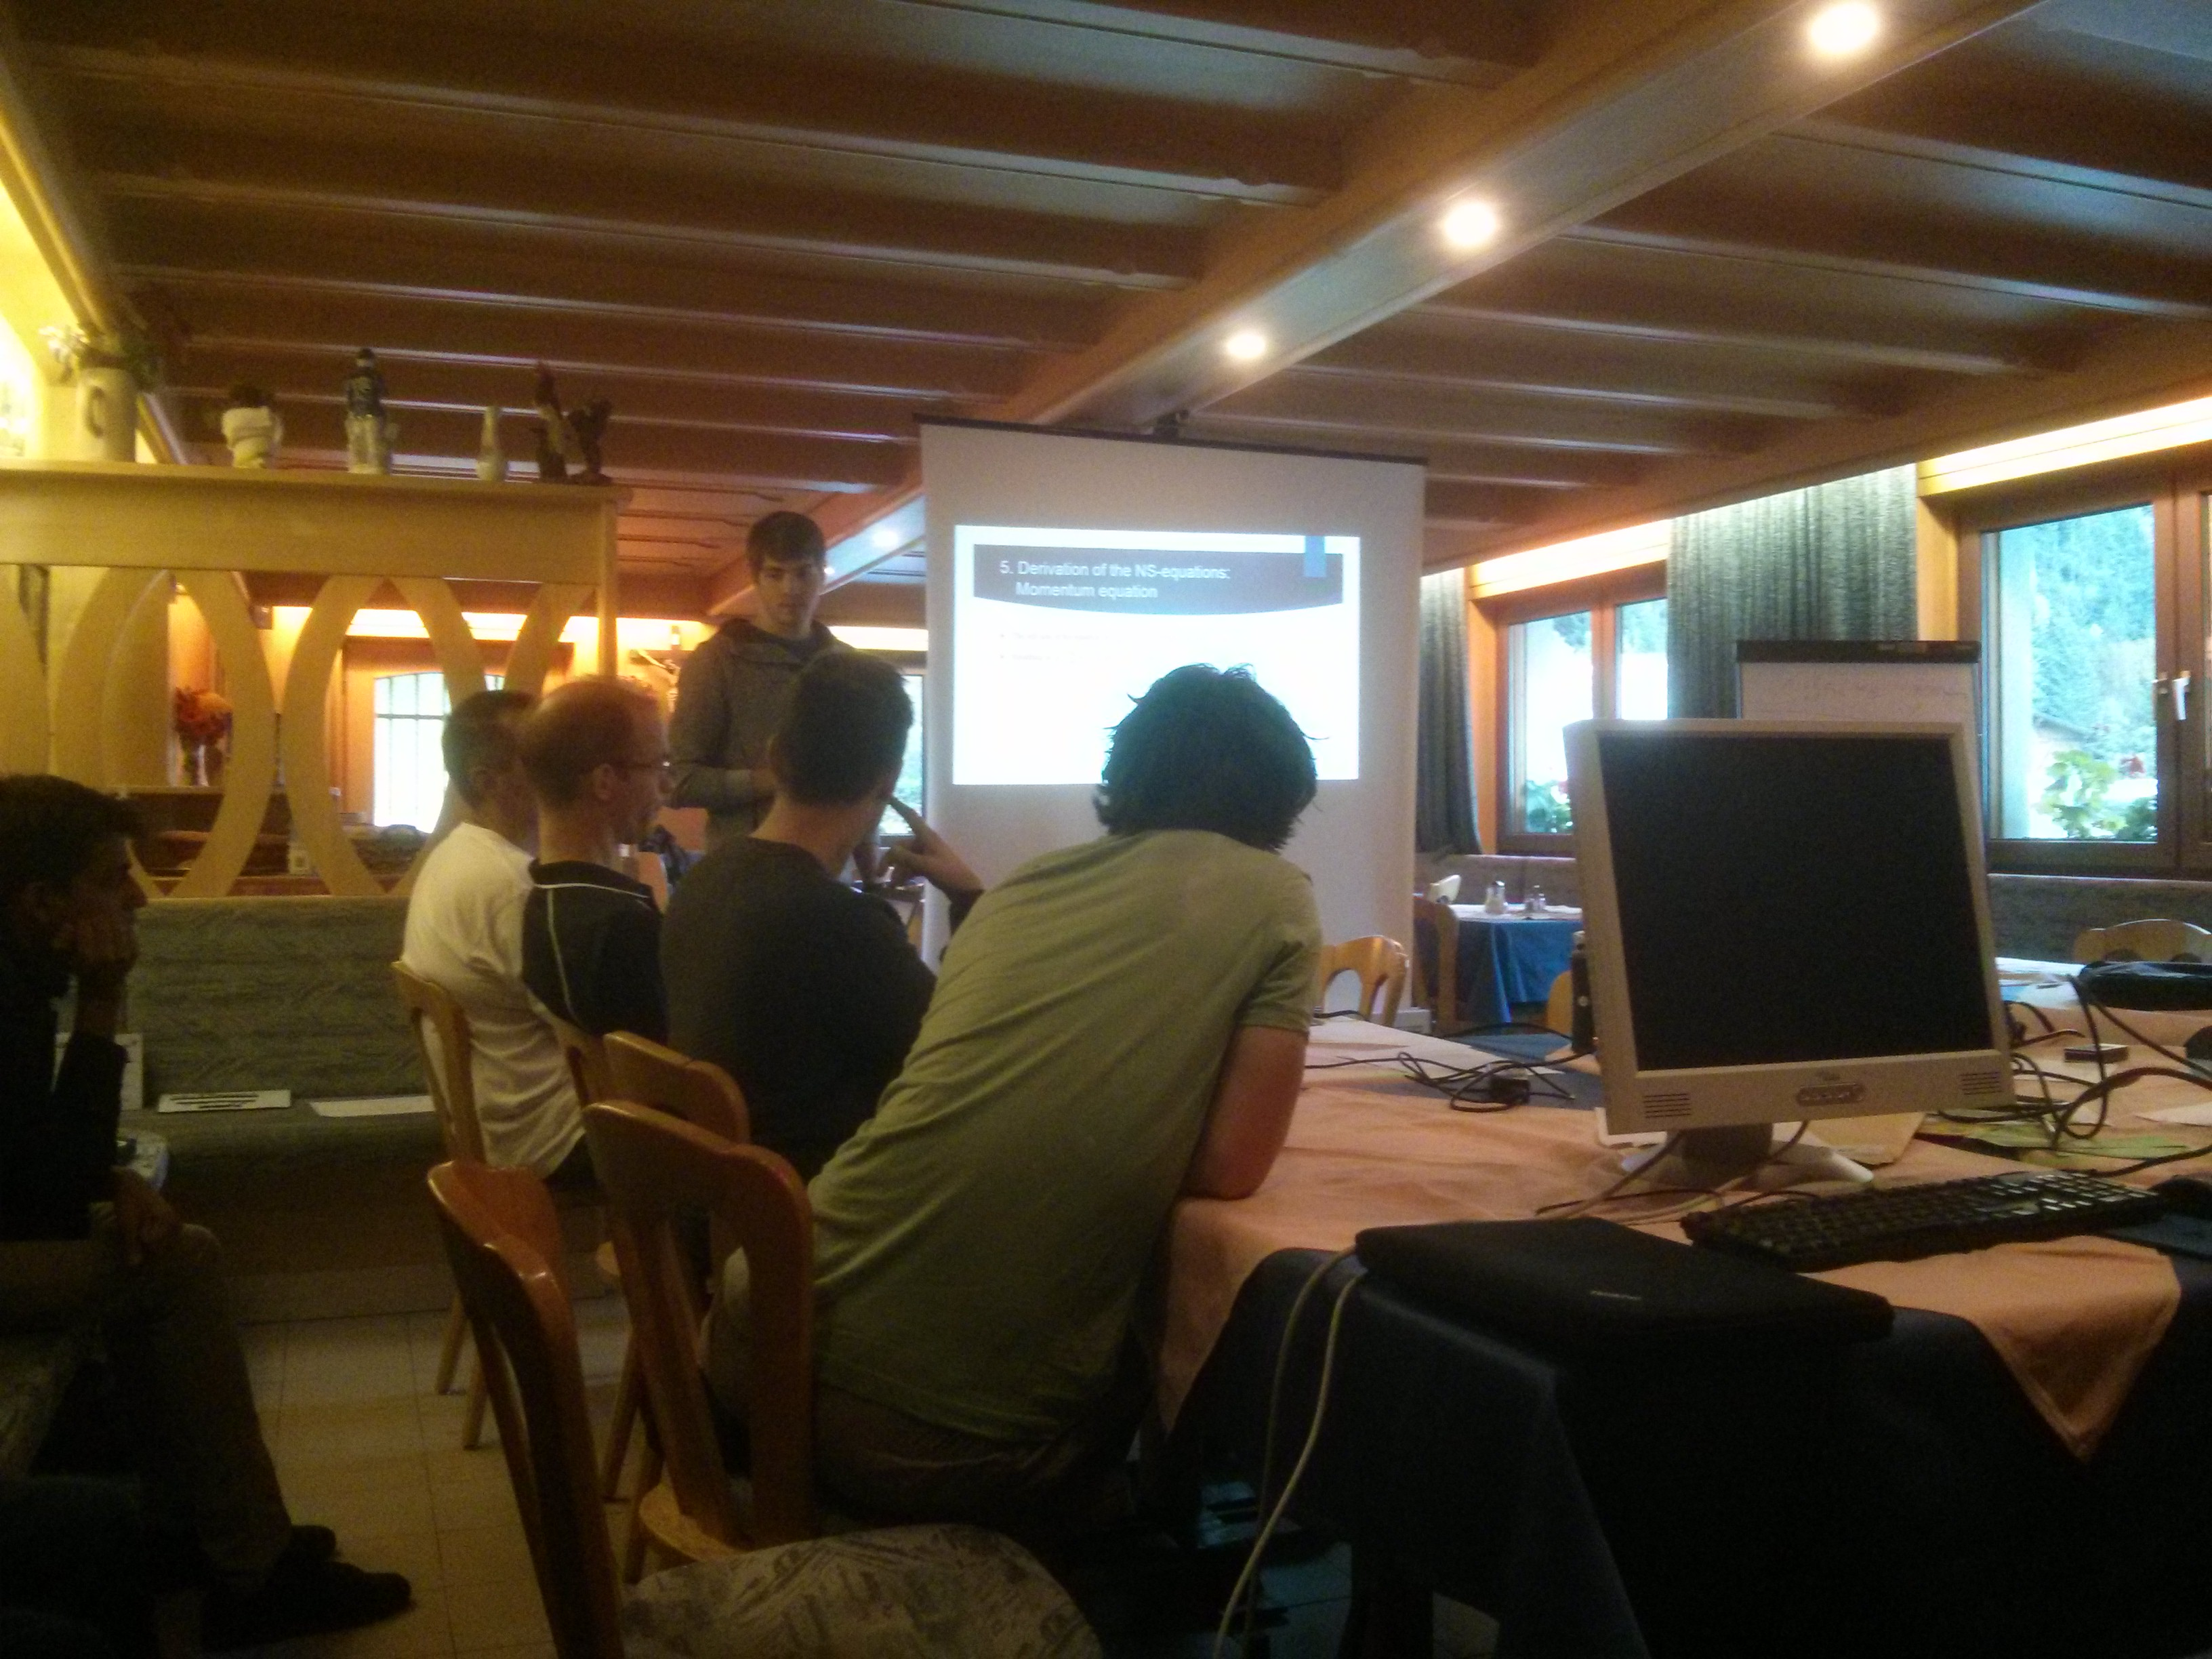
\includegraphics[scale=0.048]{img/Presentation.jpg}%
 		\caption{Presentation in a course.}\label{fig:presentation}%
 	\end{center}%
\end{figure}
\begin{figure}[ht]%
 	\begin{center}%
 		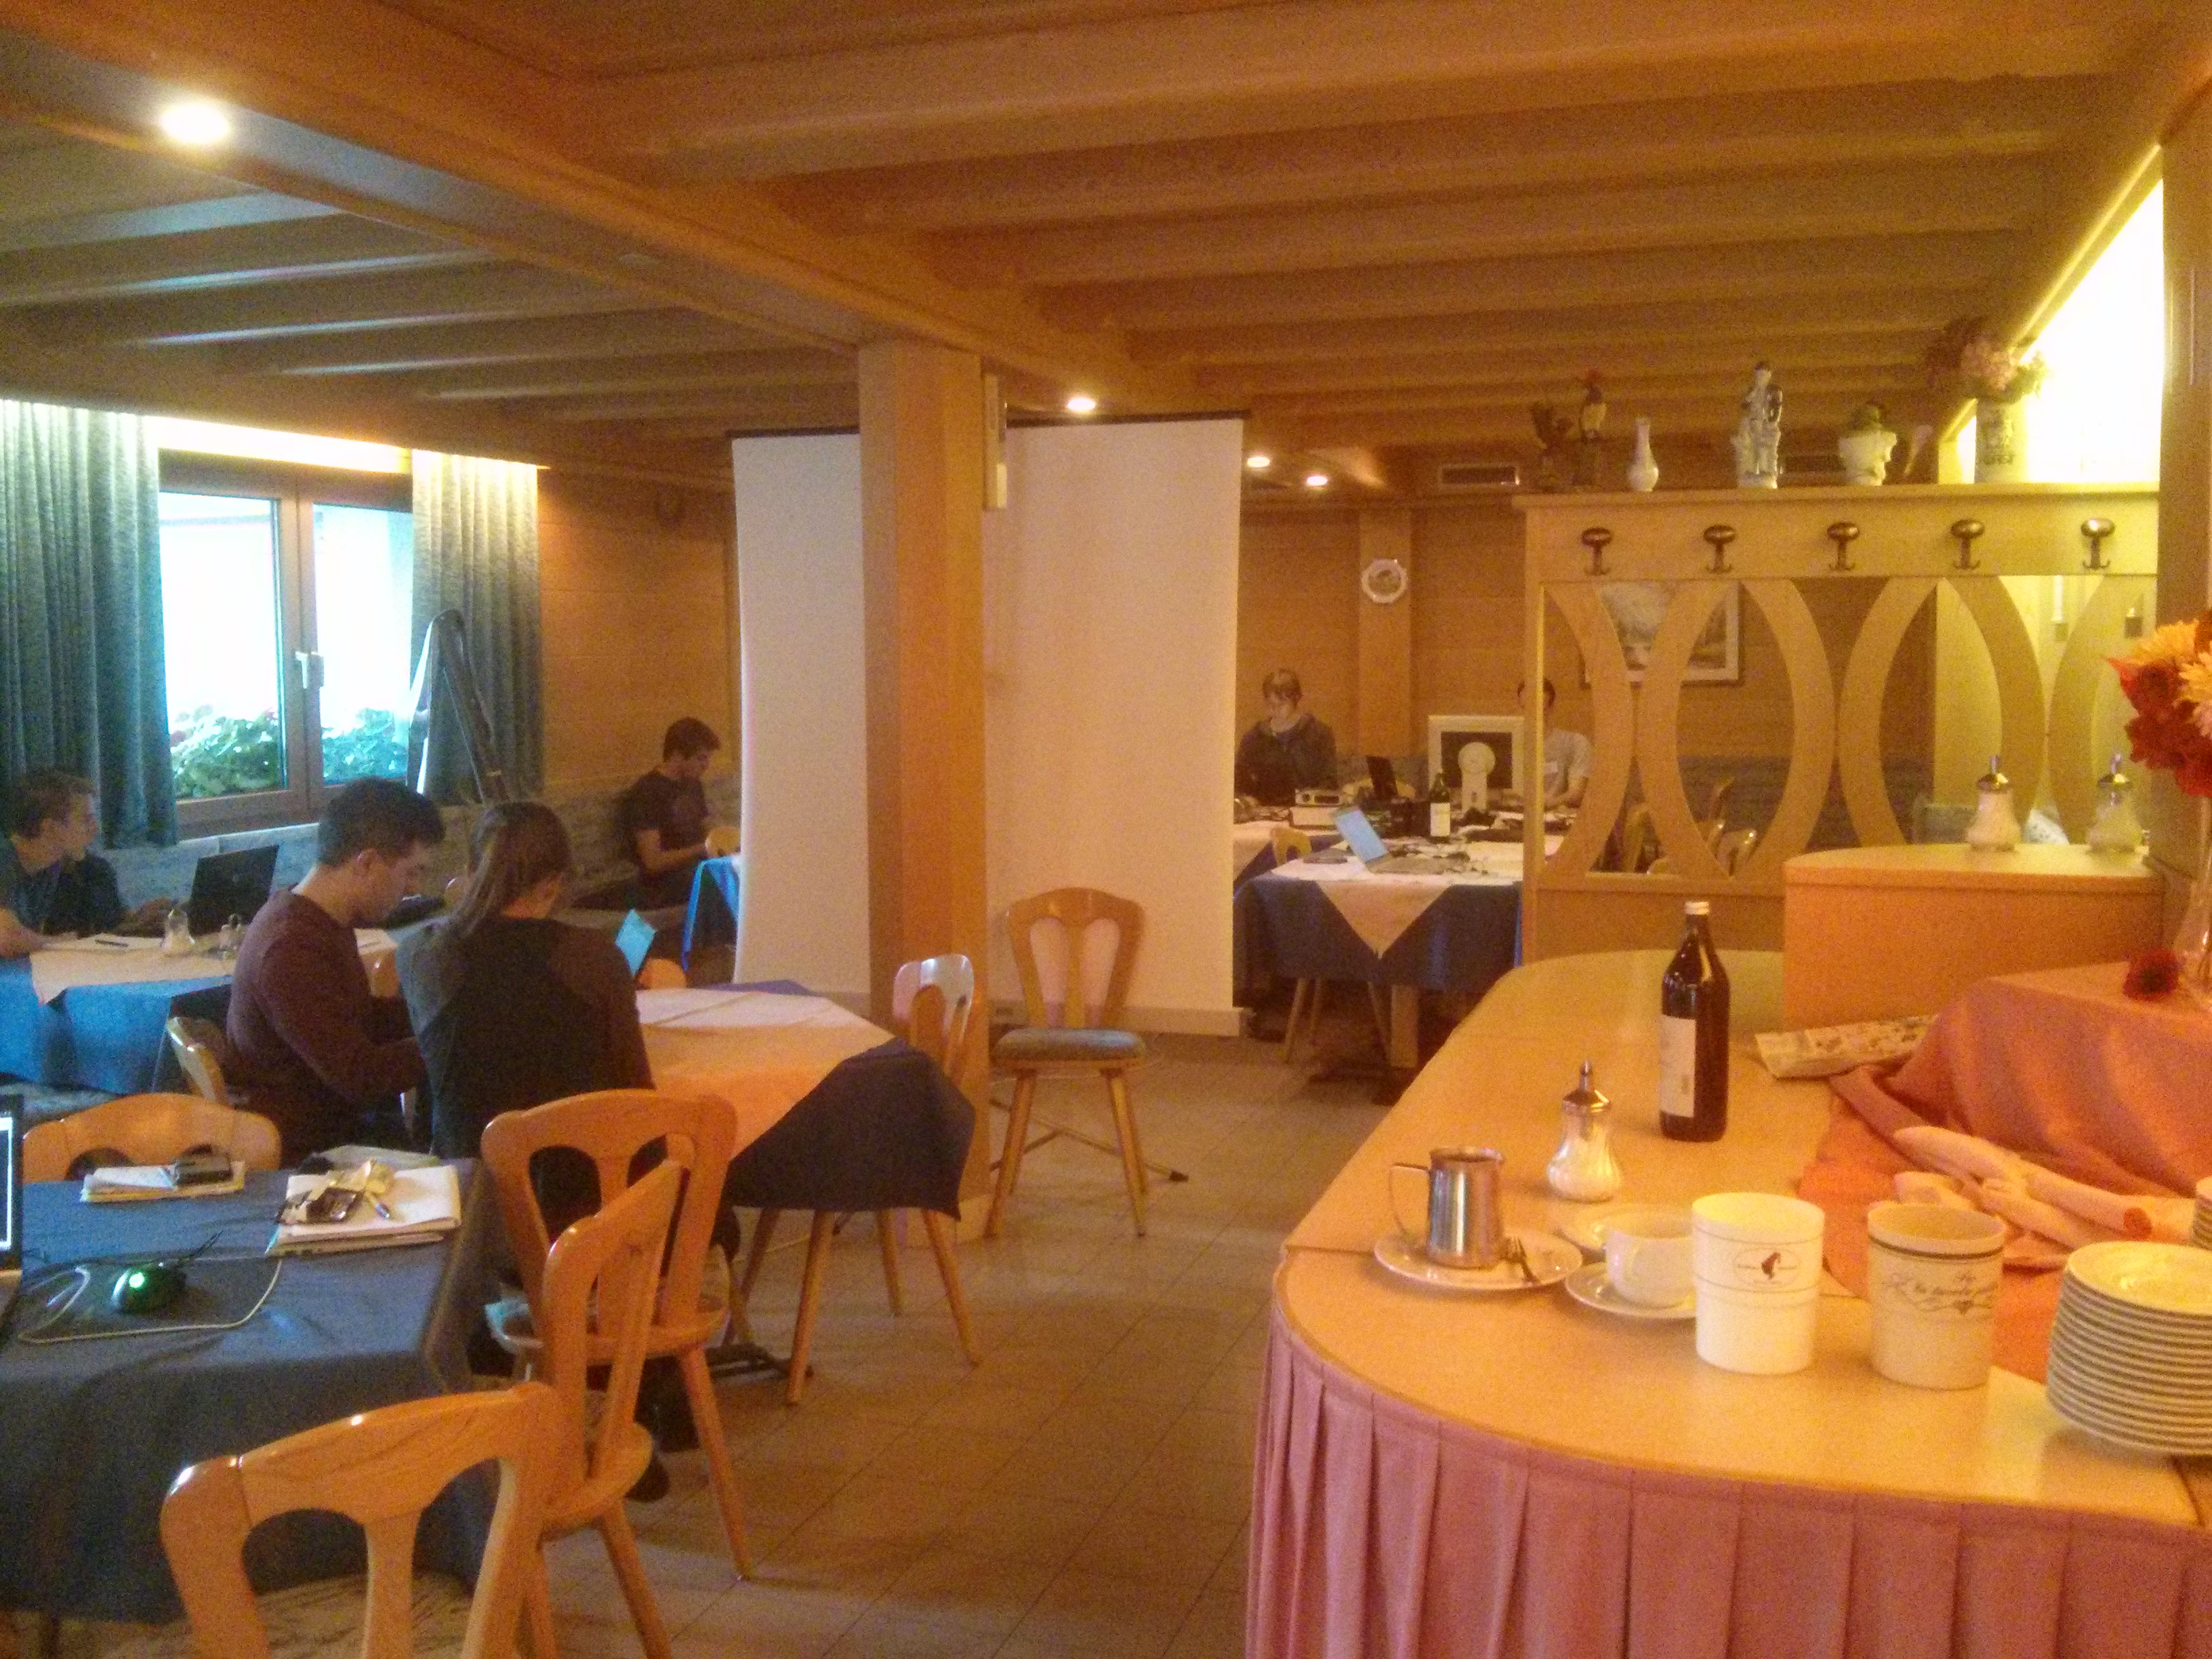
\includegraphics[scale=0.048]{img/Project.jpg}%
 		\caption{Students working on their project.}\label{fig:project}%
 	\end{center}%
\end{figure}

\begin{figure*}[ht]%
	\centering
    \begin{subfigure}[t]{0.5\textwidth}
 	\begin{center}%
 		\includegraphics[scale=0.05]{img/Hike1.jpg}%
 		%\caption{Presentation in a course.}\label{fig:hike1}%
 	\end{center}%
    \end{subfigure}%
    \begin{subfigure}[t]{0.5\textwidth}
 	\begin{center}%
 		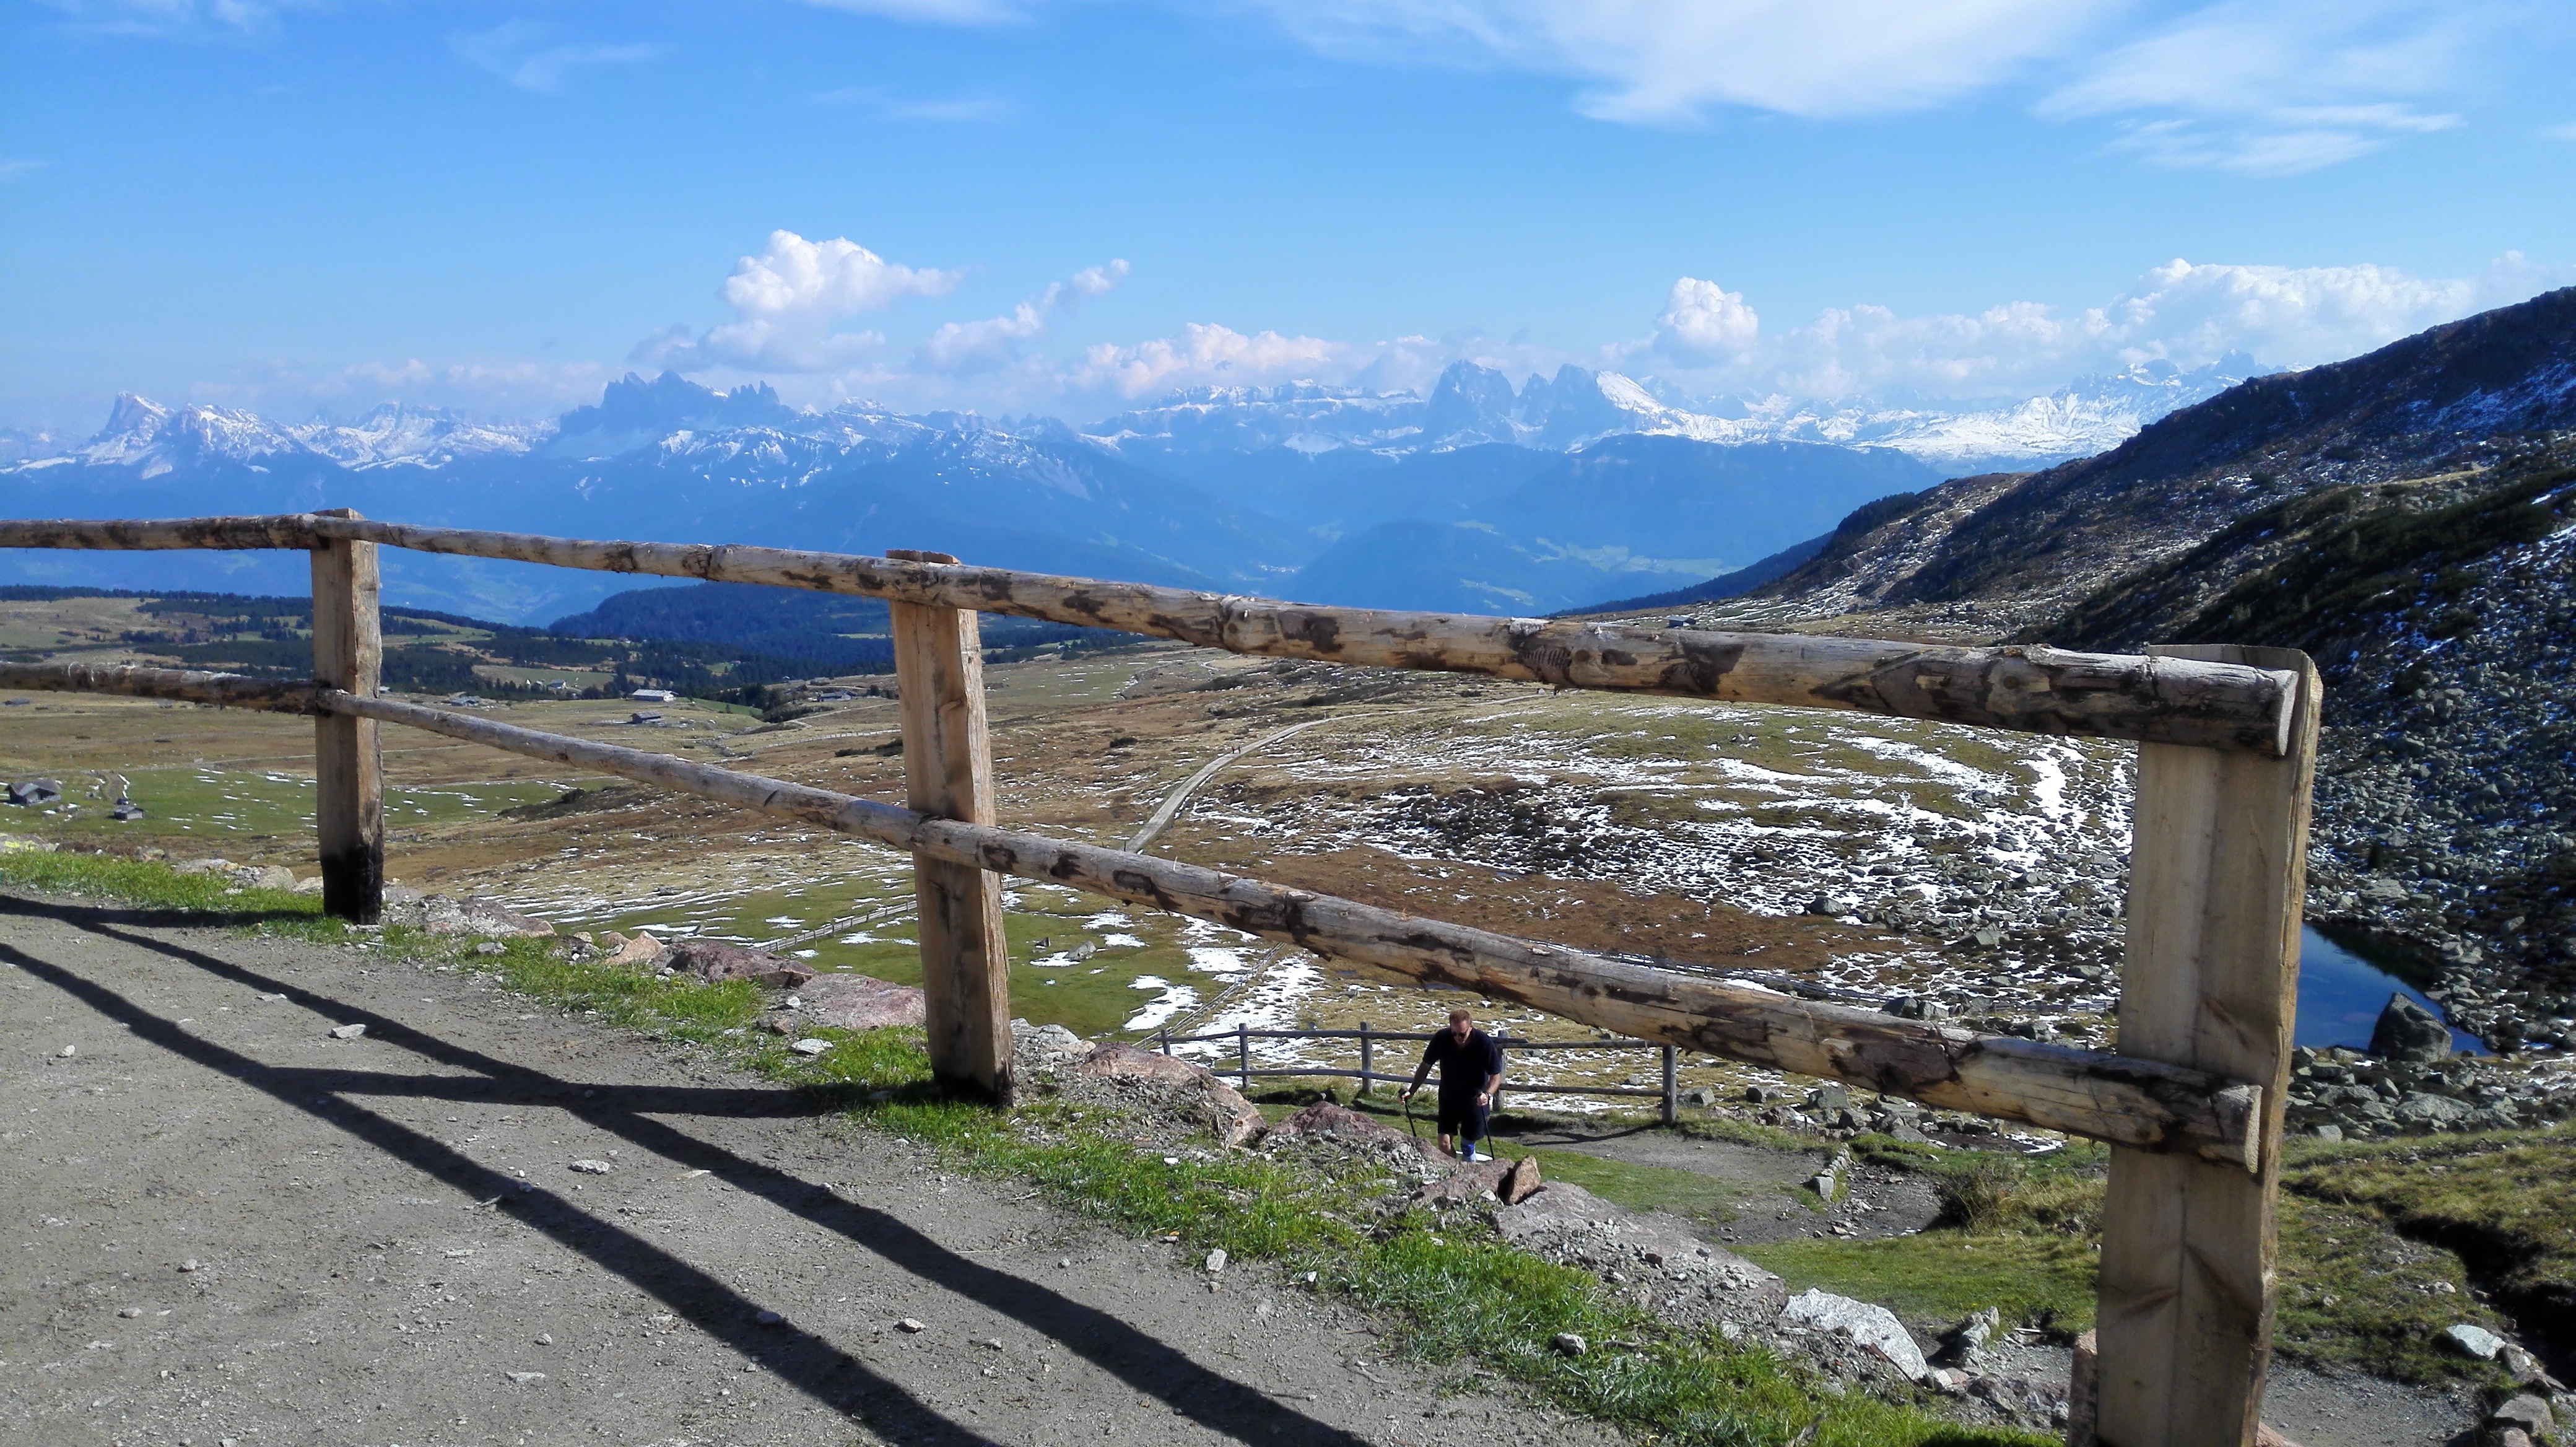
\includegraphics[scale=0.05]{img/Hike2.jpg}%
 		%\caption{Presentation in a course.}\label{fig:hike1}%
 	\end{center}%
    \end{subfigure}
    \caption{Impressions from hikes.}
    \label{fig:hiking}
\end{figure*}
\subsection{Hiking}
Right after the courses, arguably the second most important part of Ferienakademie is hiking. (Some people might even claim the hikes to be more important than the courses themselves.) Sarntal and Southern Tyrol offer a beautiful landscape in the Alps which one can explore through a number of hiking routes. While there are official hiking days (to ensure that professors do not overwhelm their students), most of the courses also plan hiking trips on their own. A healthy competitiveness evolves between the courses which culminates on the final day with the course with the most hikes being crowned \"Uberhikers (unofficially, admittedly, but there is nevertheless a lot of pride involved). Words can hardly describe the beauty of these trips, hence we refer to \autoref{fig:hiking}.

\subsection{Culture}
The cultural aspects of Sarntal play an important part at Ferienakademie. On one of the first days, all participants meet up in a local town hall and get introduced to the history and culture of Sarntal. This evening is known as "Trldieaf" (we know. "Trl-what?") which includes a presentation about the uniqueness of the valley followed by an enthralling experience of the traditional songs and clothing, see \autoref{fig:culture1}. The show concludes with a treat of the local wine (but be careful, it is not water!). 

The academy also organizes a trip to Bolzano, one of the prominent cities of South Tyrol, see \autoref{fig:culture2}. A highlight here is for example the South Tyrol Museum of Archaeology which features the Neolithic mummy "Ötzi".
\begin{figure}[ht]%
 	\begin{center}%
 		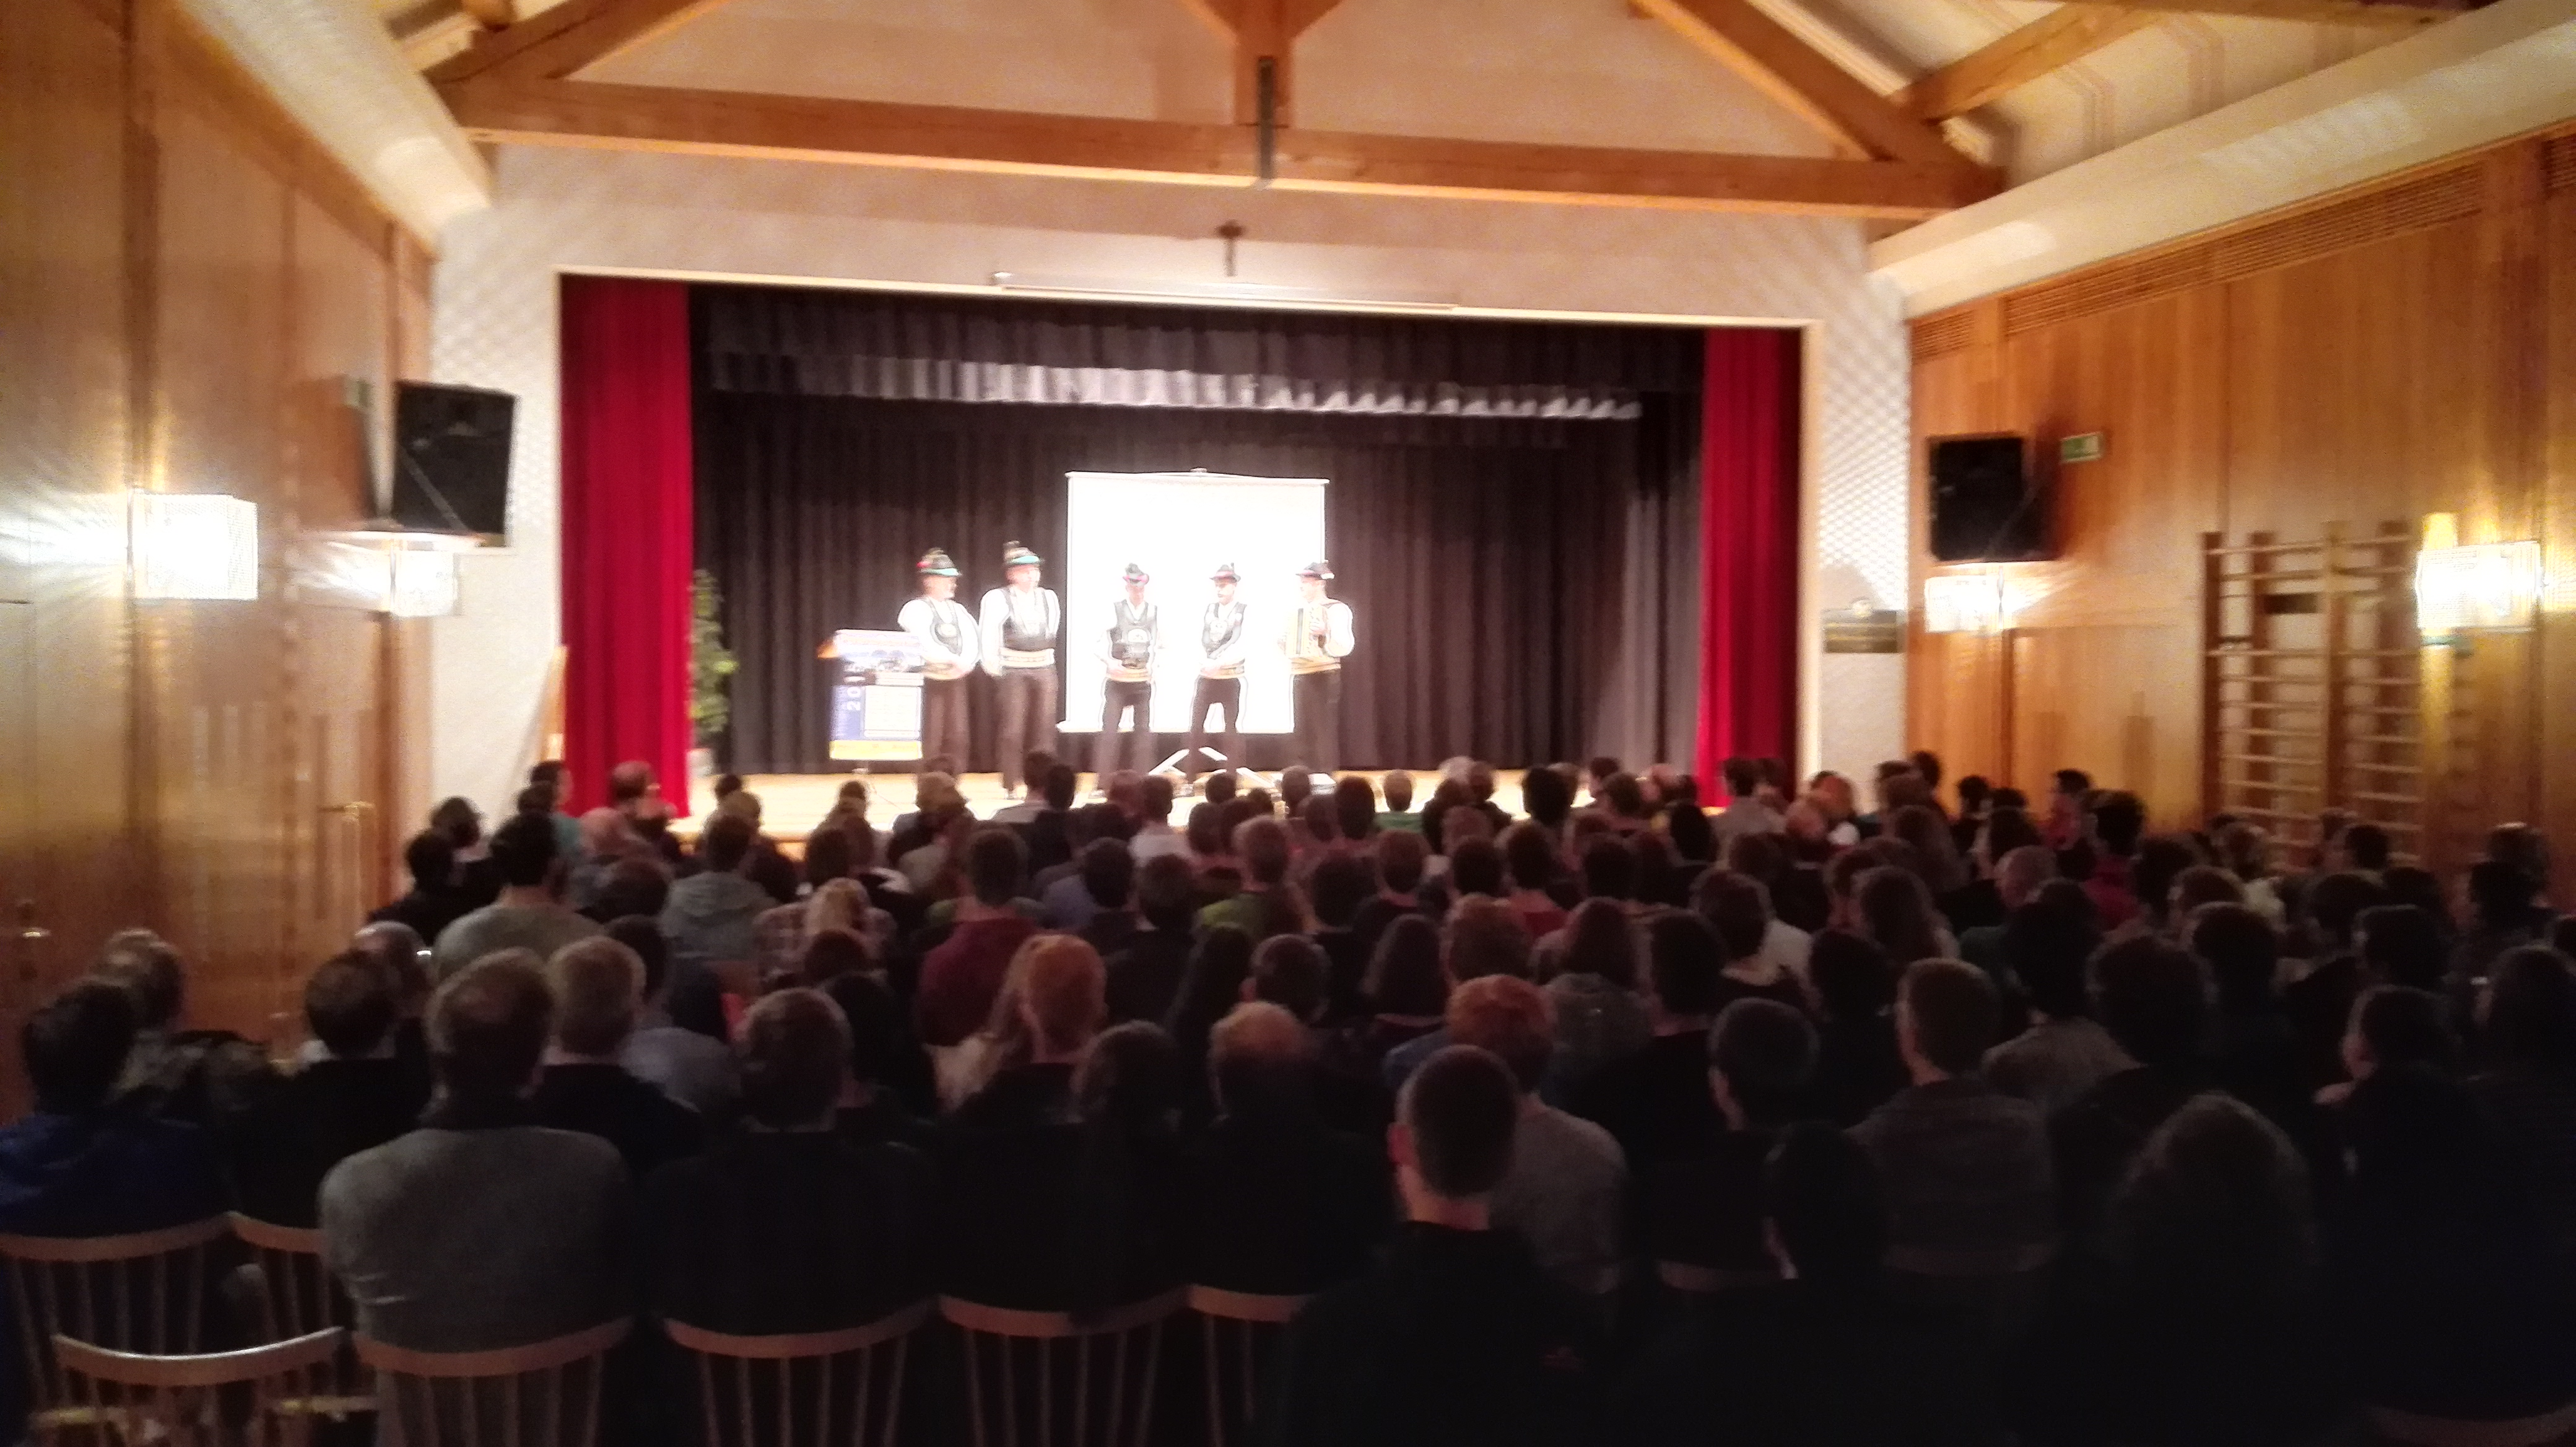
\includegraphics[scale=0.045]{img/Culture1.jpg}%
 		\caption{Trldiaf.}\label{fig:culture1}%
 	\end{center}%
\end{figure} 
\begin{figure}[ht]%
 	\begin{center}%
 		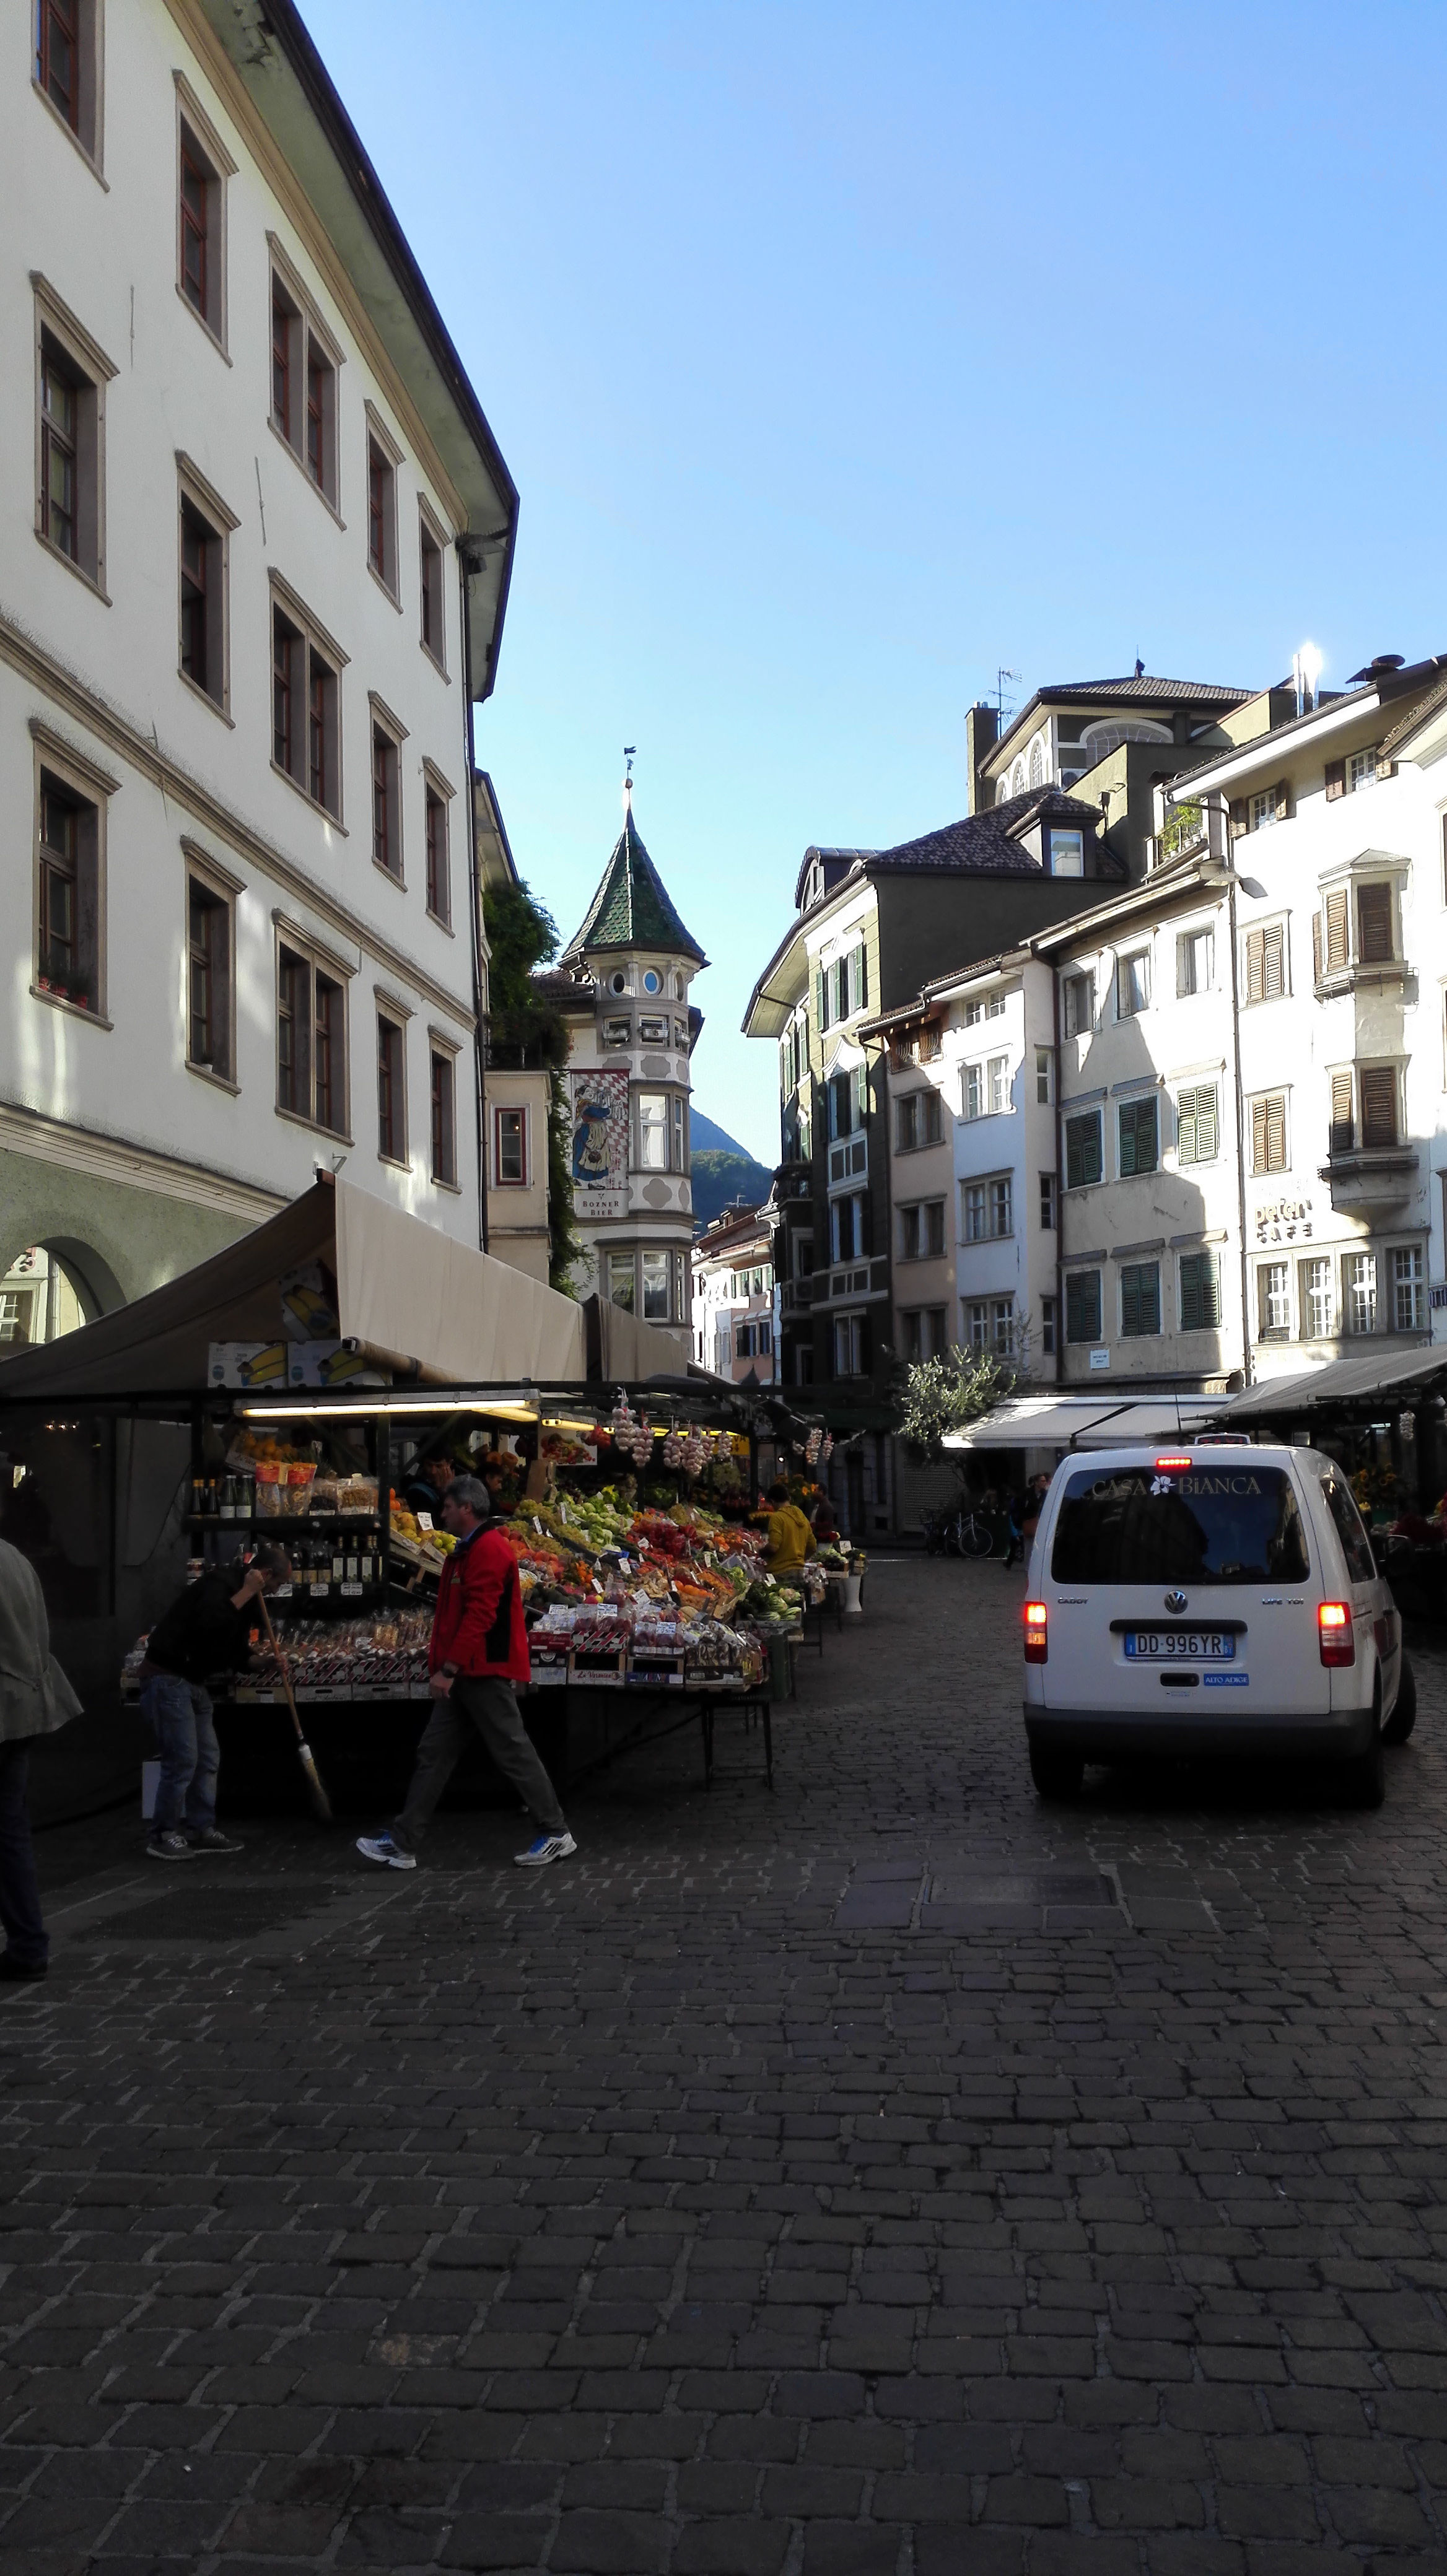
\includegraphics[scale=0.05]{img/Bolzano.jpg}%
 		\caption{Bolzano}\label{fig:culture2}%
 	\end{center}%
\end{figure} 

\subsection{Sport}
Each year three different competitions are organized for the students:
\begin{itemize}
\item Table-tennis
\item Chess
\item The Run
\end{itemize}
The table-tennis and chess competitions are held as tournaments where each house puts together a team. The houses then compete against each other in semifinals and finals. For the tournament, each team is supported in full vigor by their fans, ensuring a great atmosphere during the games (chess being the exception)-- see \autoref{fig:Tabletennis}. 
\begin{figure}[ht]%
 	\begin{center}%
 		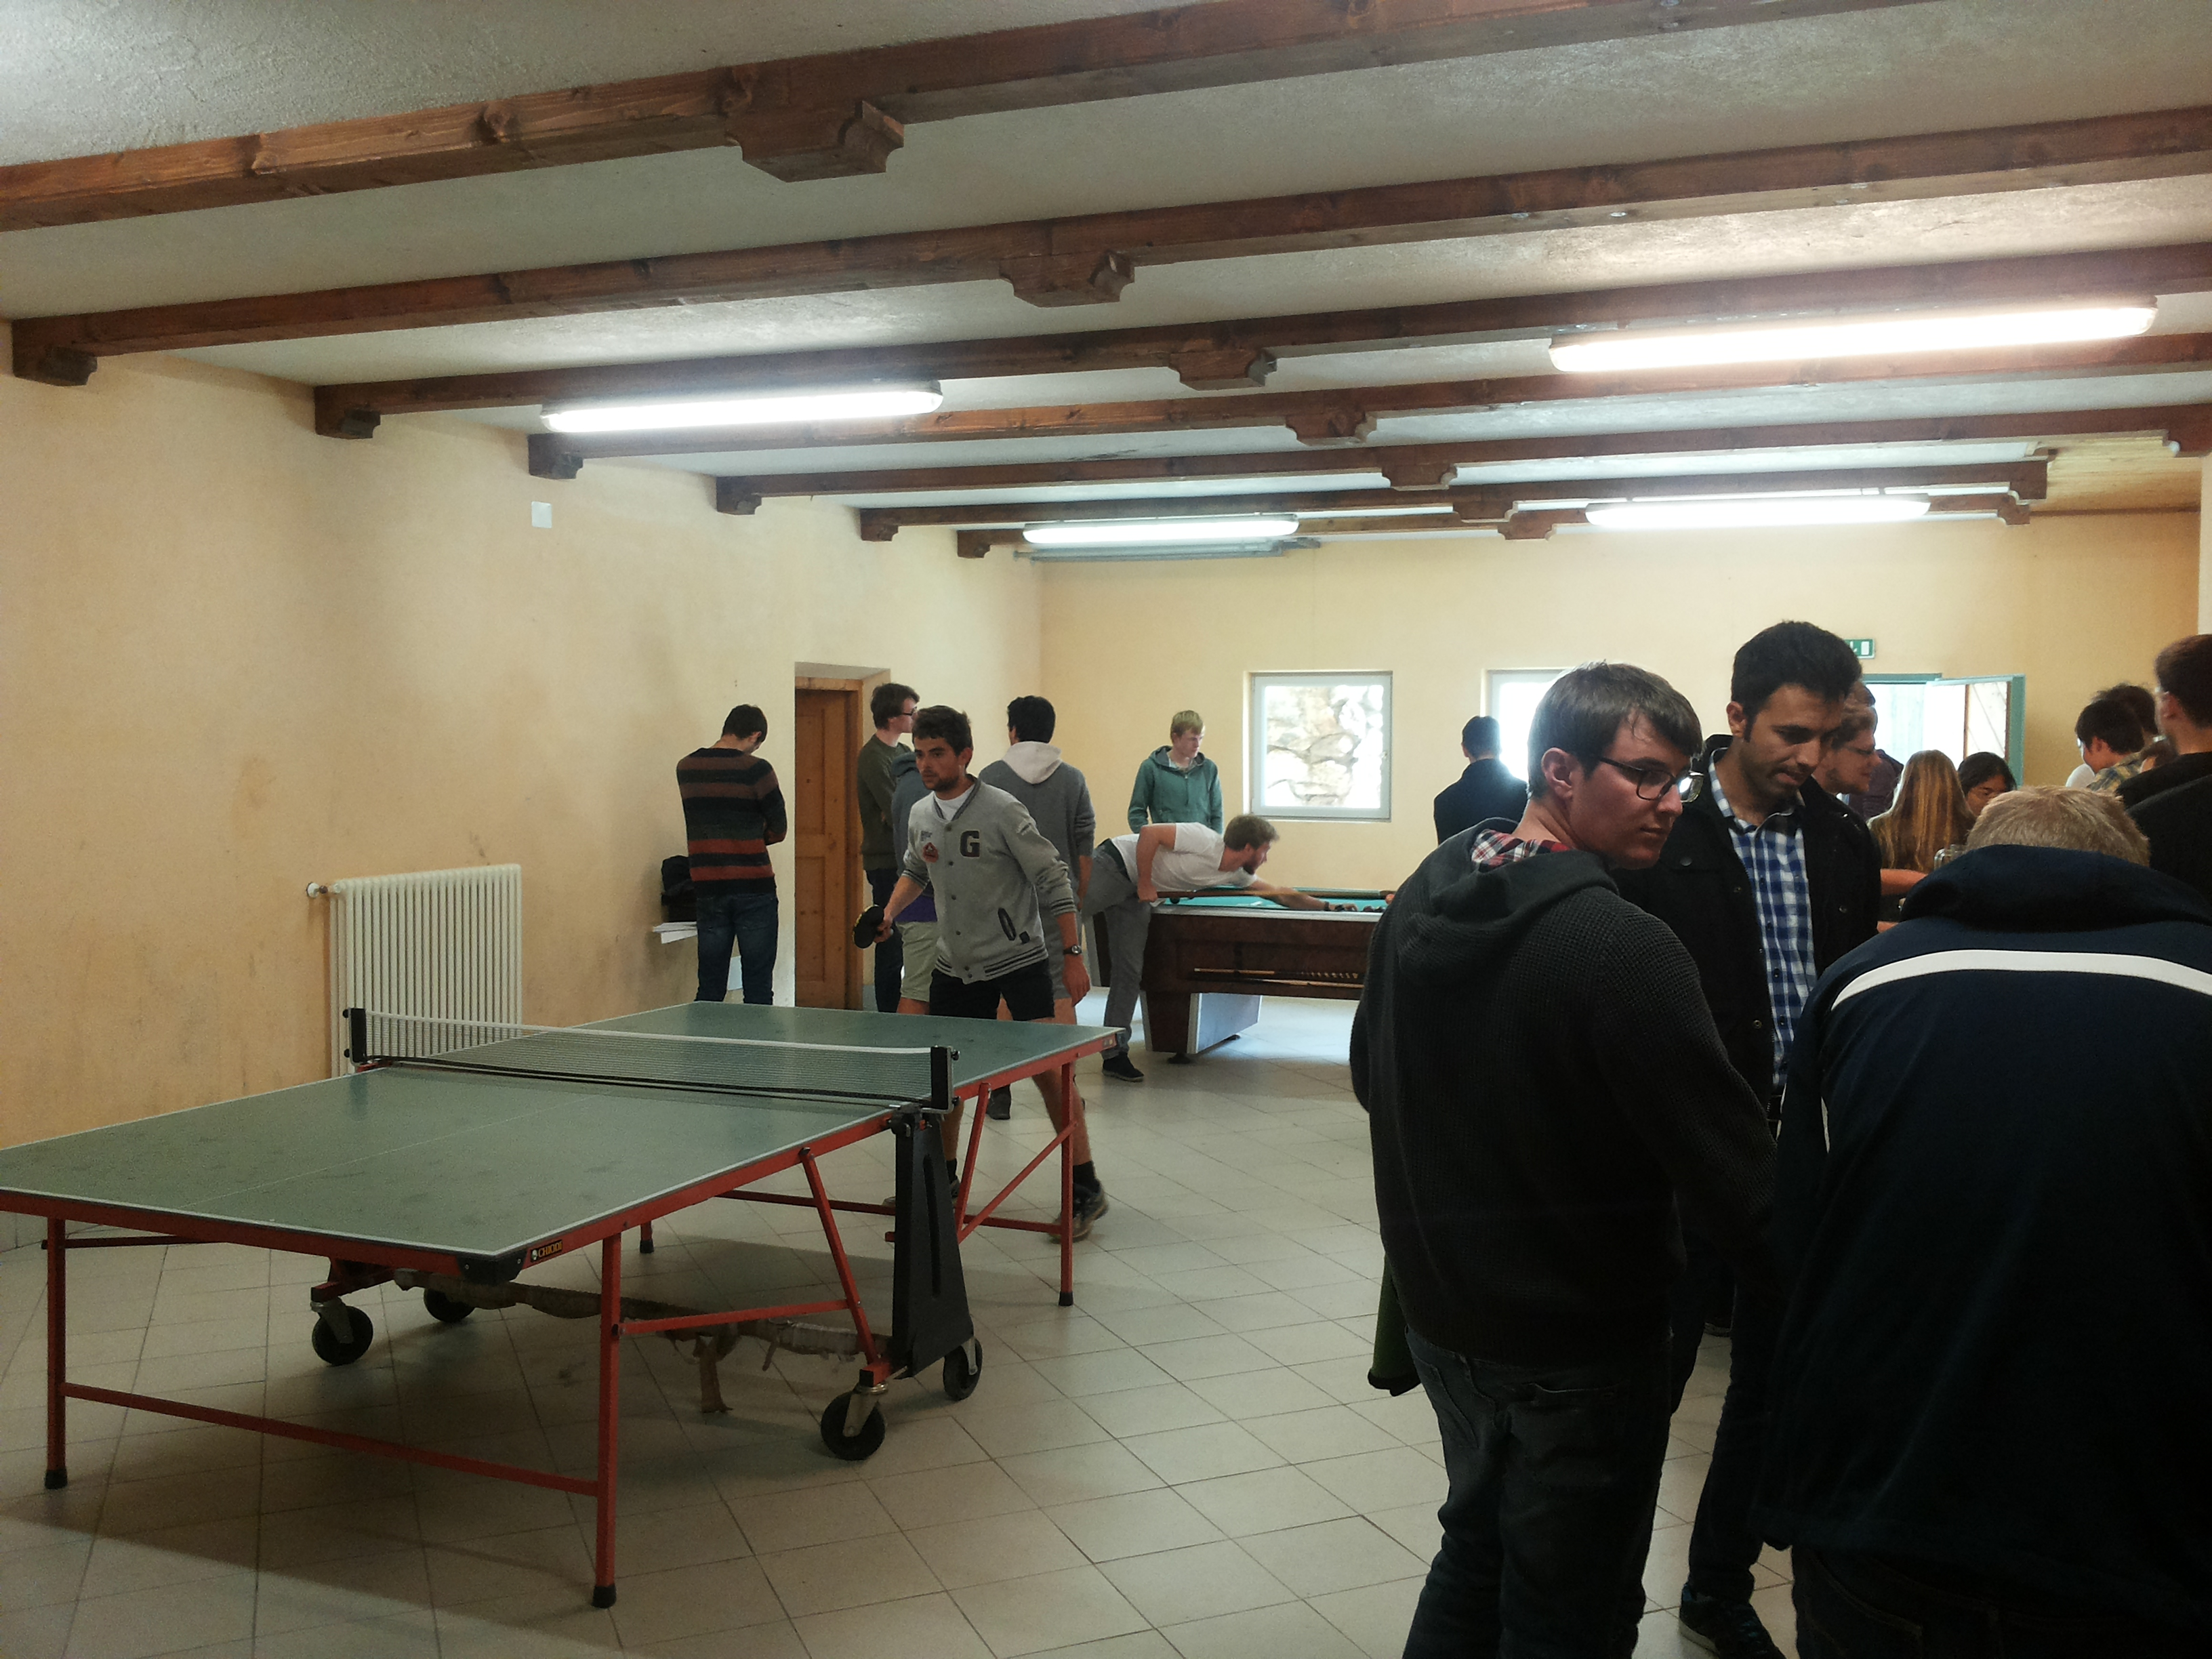
\includegraphics[scale=0.06]{img/Tabletennis.jpg}%
 		\caption{Preparing for the tabletennis tournament.}\label{fig:Tabletennis}%
 	\end{center}%
\end{figure}

The run is located at a beautiful spot, going around Lake Durnholz twice for about a total length of 4 km where the participants (and fans) can afterwards enjoy a refreshing swim in the lake. 

To show the importance of these activities, it is said, that some professors value the result of the tournaments higher than the results in the actual courses.

\subsection{Food}
Last, but not the least, the food. Despite the physical demands of the hikes (some courses hike more than fifty kilometers) [reference needed] and intellectual toll of the courses, no on returns from Ferienakademie with a loss in weight. Culinary delights at Ferienakademie are a-plenty! The choice ranges from a sumptous noodle buffet to an array of dumplings; from schnitzel to Jause. And then there is Kaiserschmarrn. If you have never been in the gourmet heaven called Kaiserschmarrn, wait for Ferienakademie. Not only is it mandatory to eat at every hut you take a break during hikes; there is also a special Kaiserschmarrn-evening where the students try to eat the kitchen empty-- literally. Prof. Bungartz likes to tell the story of Feldrand having to buy eggs from a neighbouring farm to provide more Kaiserschmarrn for the hungry students. The beauty and instant-appetizing nature a plate of Kaiserschmarrn is illustrated in \autoref{fig:Kaiserschmarrn}.
\begin{figure}[ht]%
 	\begin{center}%
 		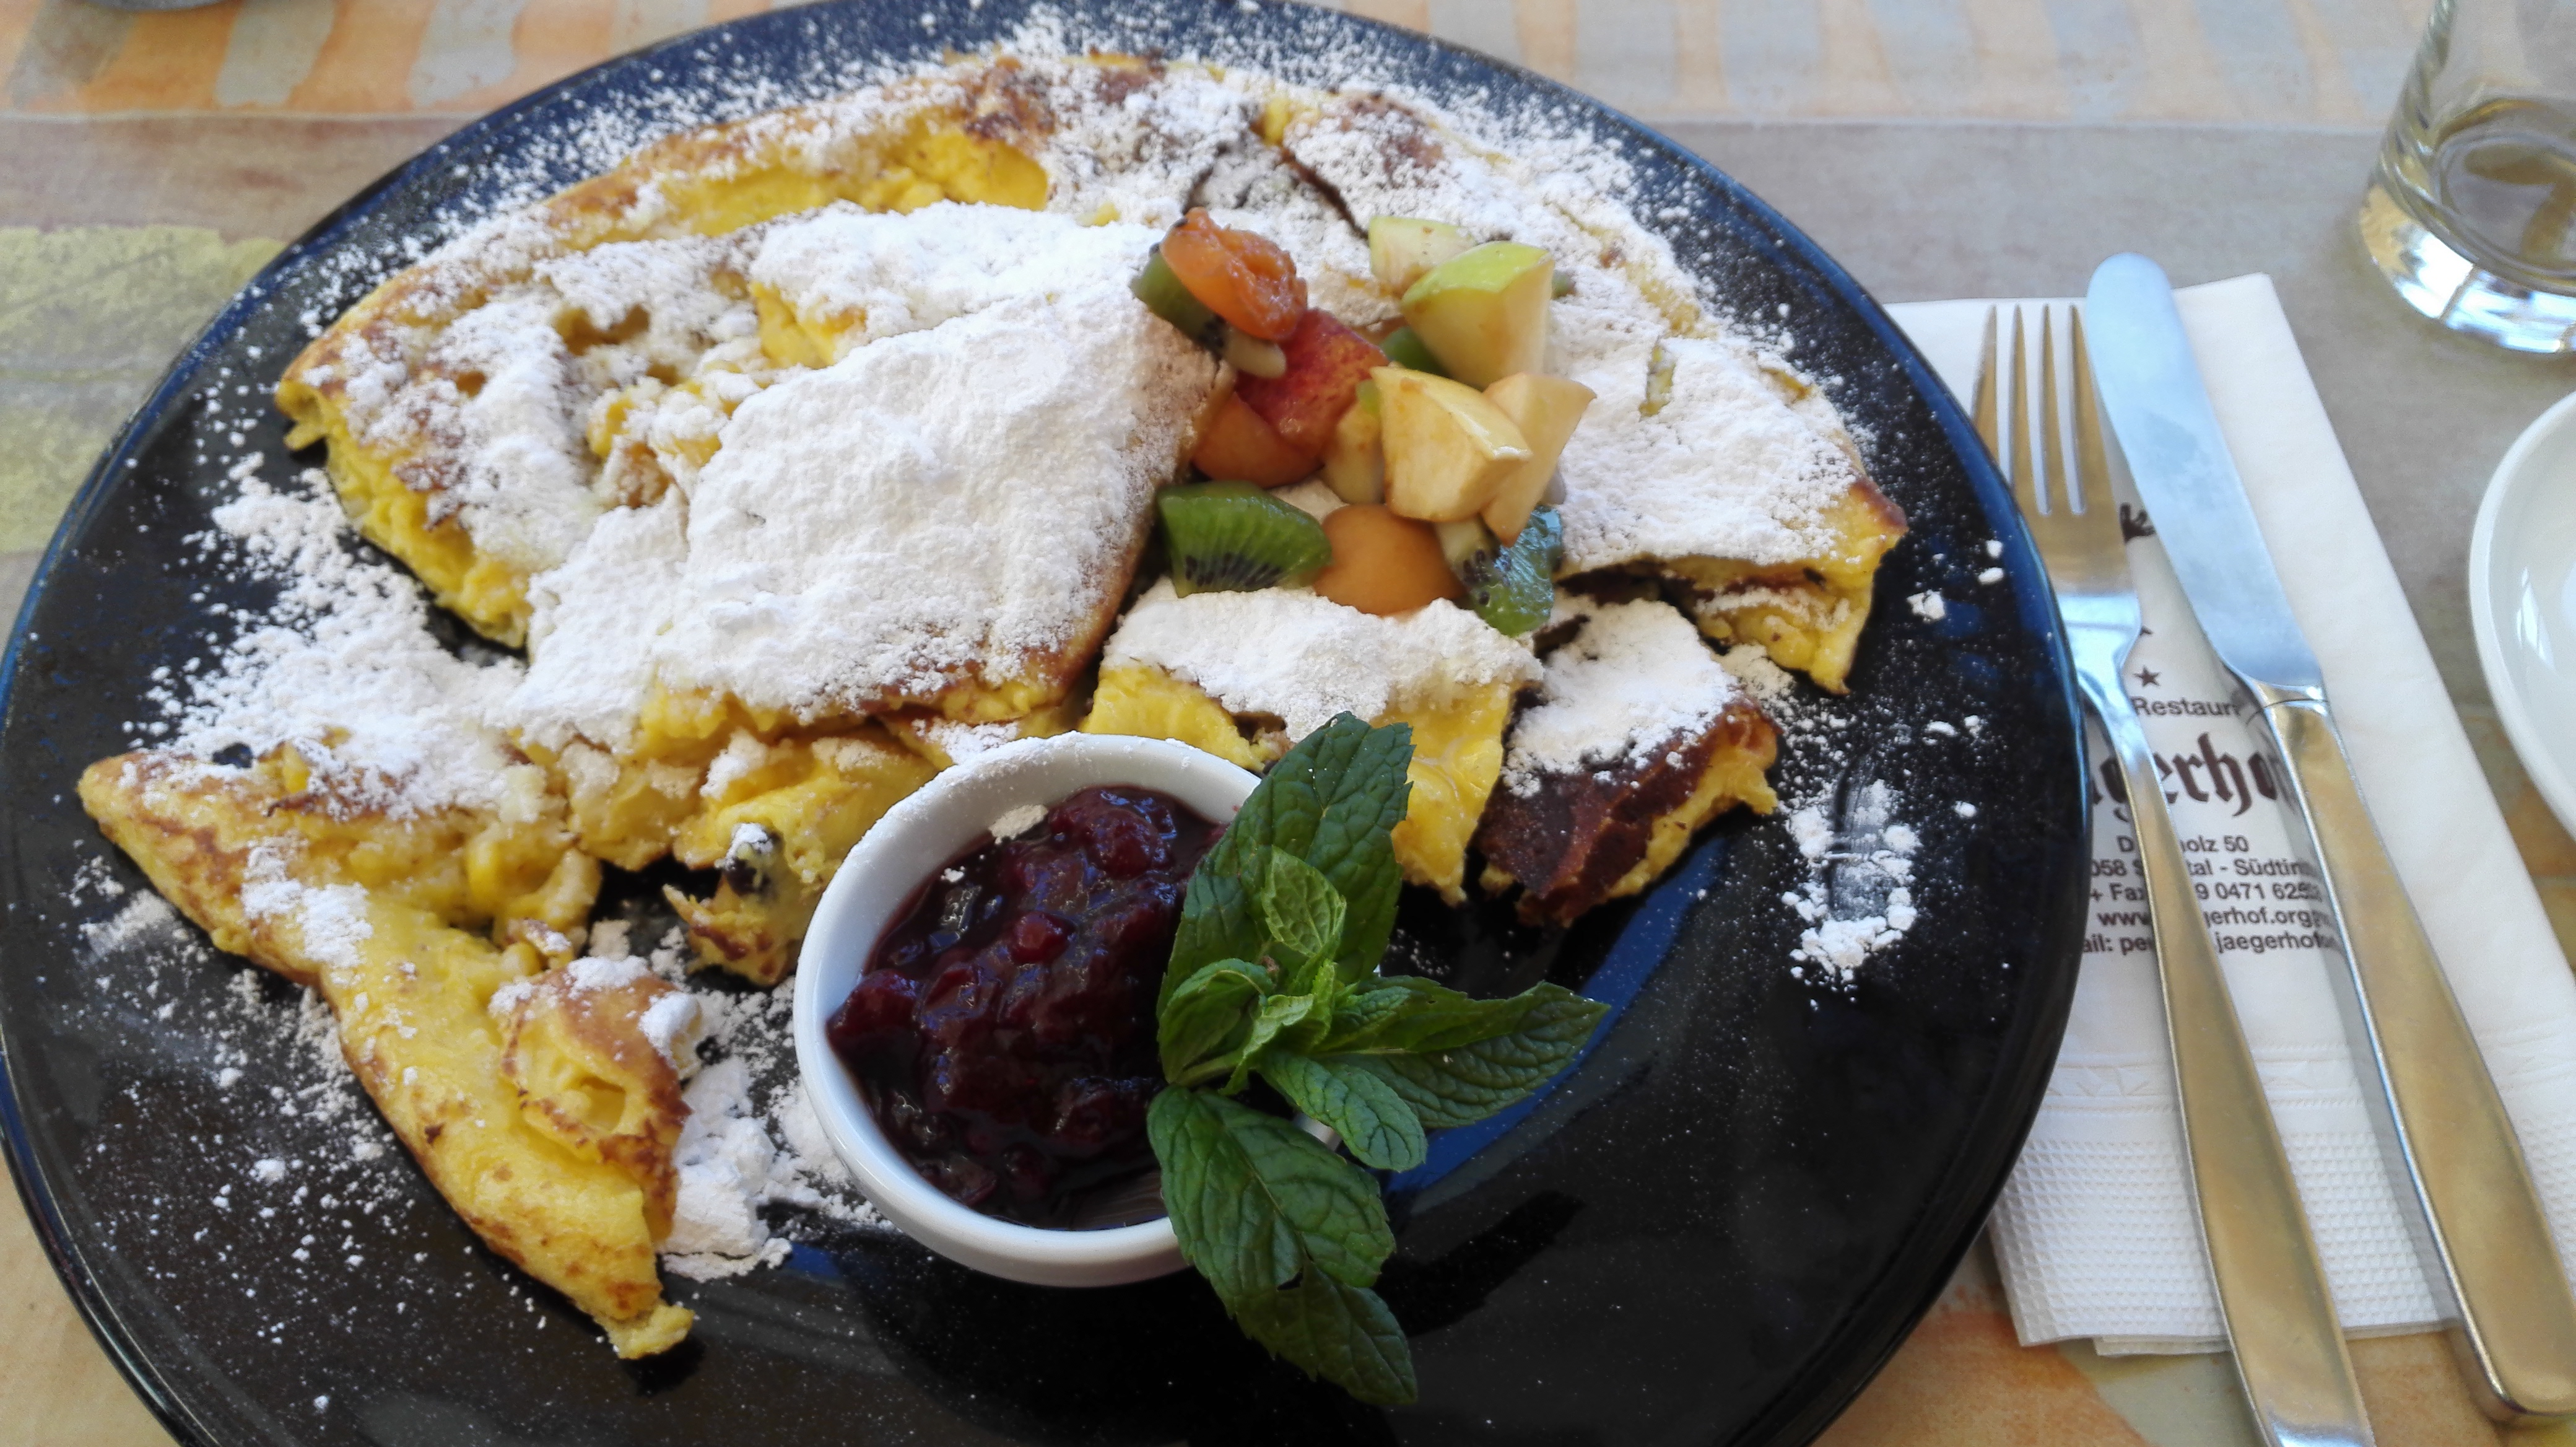
\includegraphics[scale=0.05]{img/Kaiserschmarrn.jpg}%
 		\caption{Kaiserschmarrn [Jägerhof et al.]}\label{fig:Kaiserschmarrn}%
 	\end{center}%
\end{figure}

During our stay at Ferienakademie, we ended up developing a love for Kaiserschmarrn which we would like to express by the following poem-- Ode an den Kaiserschmarrn (with the rhythm of Friedrich Schiller's "Ode an die Freude"). 
\begin{figure}[ht]
\begin{framed}
An den Kaiserschmarrn 
\\
\\
%\begin{small}
Freude, leck'rer Kaiserschmarren,\\
Mehlspeis mit Rosinen,\\
Wir verspeisen wie Barbaren \\
hunderte Portionen.\\

Jede Wand'rung endet wieder \\
mit nem Blech voll Kaiserschmarrn.\\
Studenten, die am meisten essen,\\
die sieht Bungartz voll stolz an.
%\end{small}
\end{framed}
\end{figure}
\vfill
%\columnbreak
